\documentclass{standalone}
\usepackage{tikz}
\usetikzlibrary{patterns, positioning}
\usepackage[sfdefault]{ClearSans} %% option 'sfdefault' activates Clear Sans as the default text font
\usepackage[T1]{fontenc}

\begin{document}
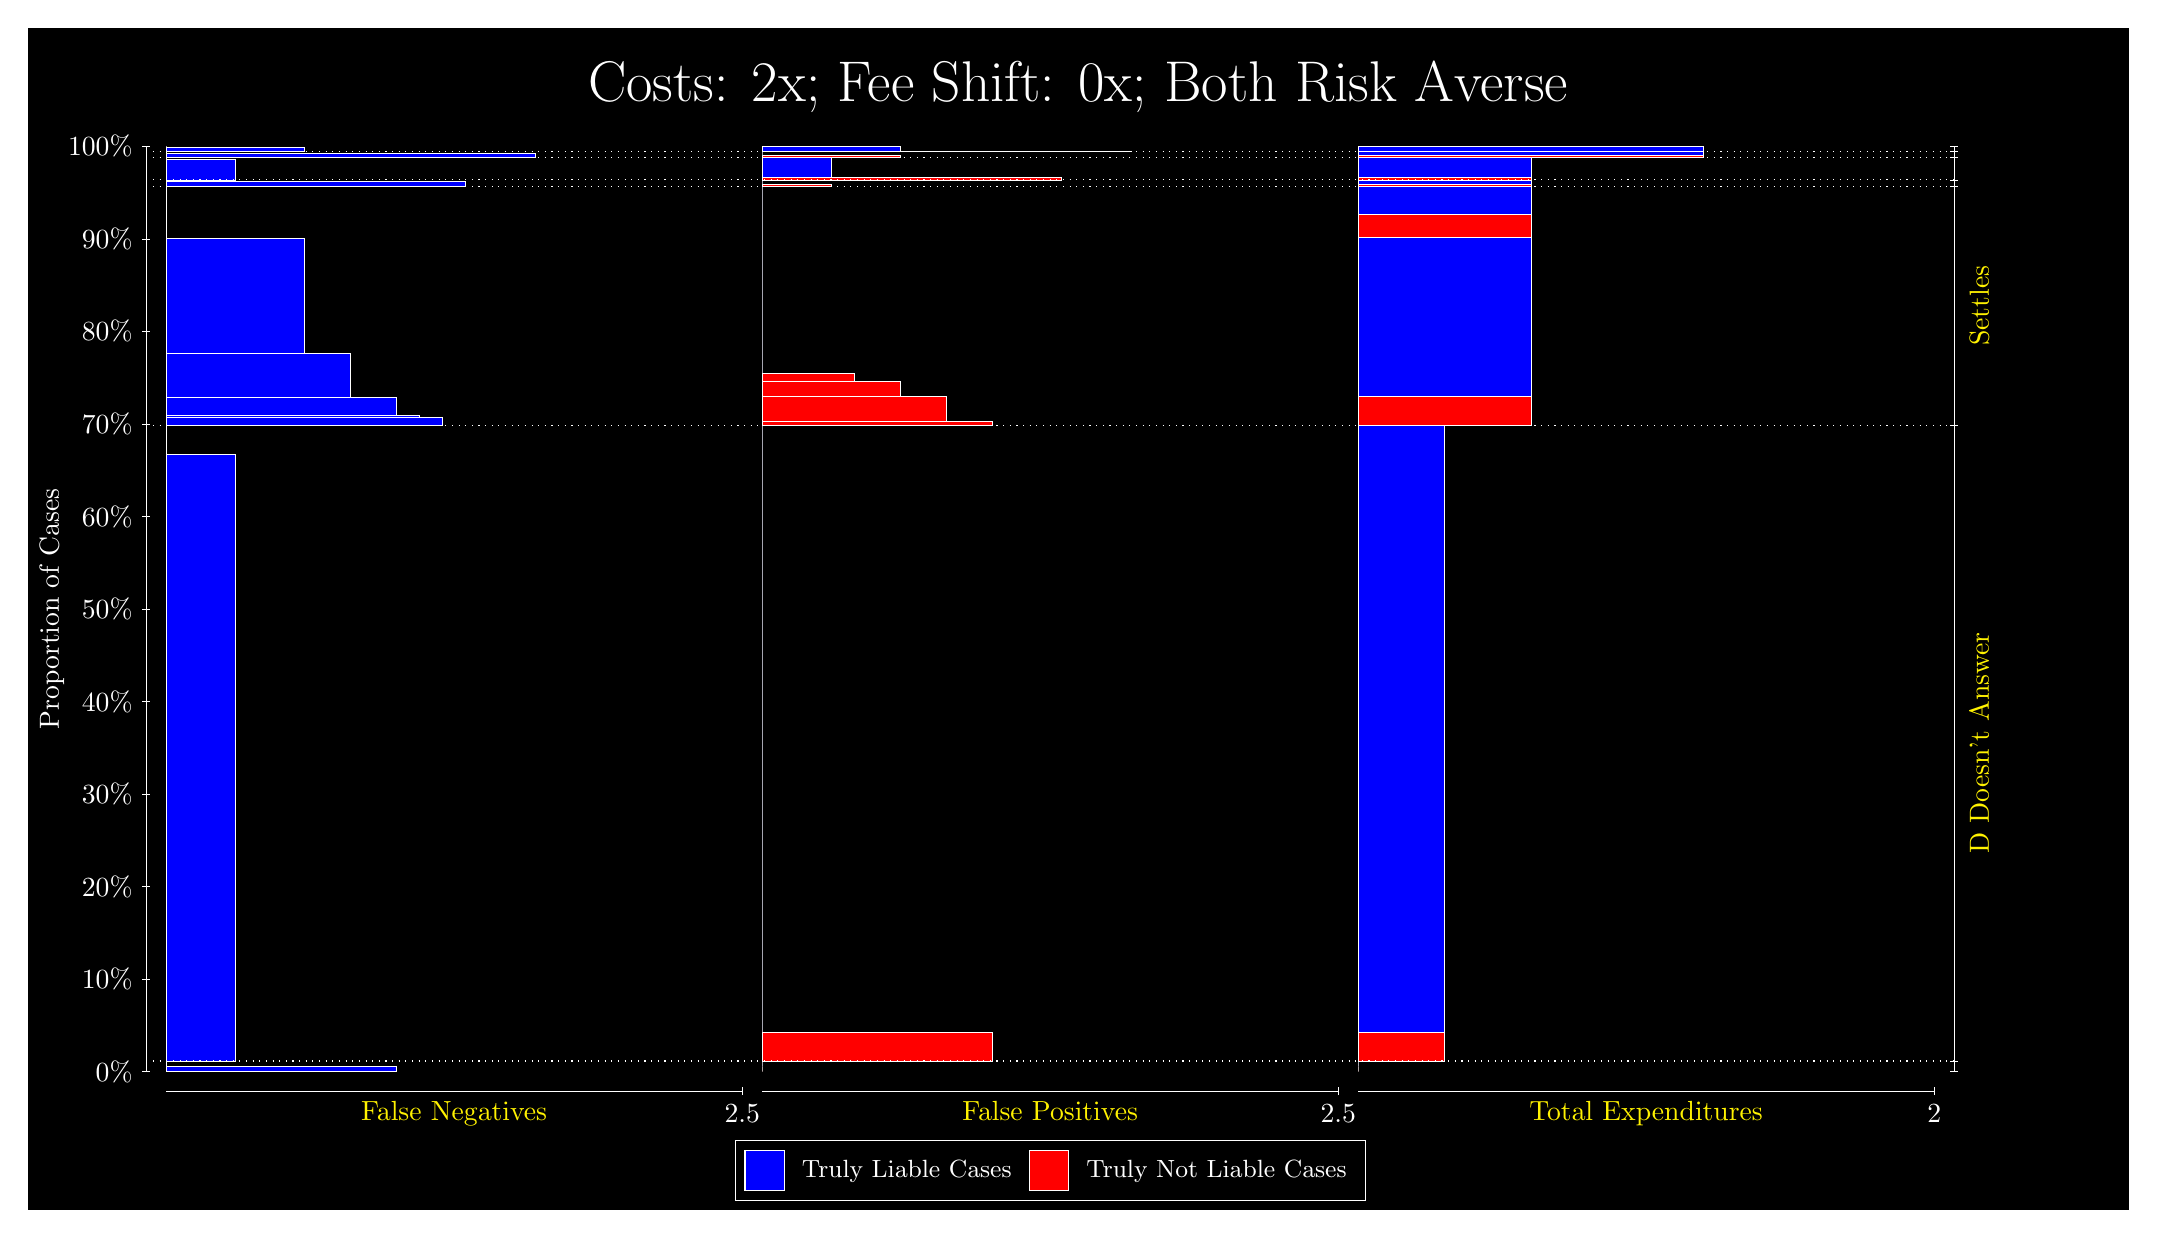
\begin{tikzpicture}
\draw[fill=black] (0,0) rectangle (26.667,15);
\draw[text=white] (0,13.5) rectangle (26.667,15) node[midway] {\huge Costs: 2x; Fee Shift: 0x; Both Risk Averse};
\draw[white, very thin] (1.5,1.75) -- (1.5,13.5);
\node[rotate=90, text=white, anchor=center] at (0.3, 7.625) {Proportion of Cases};
\draw[white, very thin] (1.45,1.75) -- (1.55,1.75);
\node[text=white, anchor=east] at (1.45, 1.75) {0\%};
\draw[white, very thin] (1.45,2.925) -- (1.55,2.925);
\node[text=white, anchor=east] at (1.45, 2.925) {10\%};
\draw[white, very thin] (1.45,4.1) -- (1.55,4.1);
\node[text=white, anchor=east] at (1.45, 4.1) {20\%};
\draw[white, very thin] (1.45,5.275) -- (1.55,5.275);
\node[text=white, anchor=east] at (1.45, 5.275) {30\%};
\draw[white, very thin] (1.45,6.45) -- (1.55,6.45);
\node[text=white, anchor=east] at (1.45, 6.45) {40\%};
\draw[white, very thin] (1.45,7.625) -- (1.55,7.625);
\node[text=white, anchor=east] at (1.45, 7.625) {50\%};
\draw[white, very thin] (1.45,8.8) -- (1.55,8.8);
\node[text=white, anchor=east] at (1.45, 8.8) {60\%};
\draw[white, very thin] (1.45,9.975) -- (1.55,9.975);
\node[text=white, anchor=east] at (1.45, 9.975) {70\%};
\draw[white, very thin] (1.45,11.15) -- (1.55,11.15);
\node[text=white, anchor=east] at (1.45, 11.15) {80\%};
\draw[white, very thin] (1.45,12.325) -- (1.55,12.325);
\node[text=white, anchor=east] at (1.45, 12.325) {90\%};
\draw[white, very thin] (1.45,13.5) -- (1.55,13.5);
\node[text=white, anchor=east] at (1.45, 13.5) {100\%};

\draw[white, very thin] (24.457,1.75) -- (24.457,13.5);
\draw[white, very thin] (24.407,1.75) -- (24.507,1.75);
\node[anchor=west] at (24.407, 1.75) {};
\draw[white, very thin] (24.407,1.8842) -- (24.507,1.8842);
\node[anchor=west] at (24.407, 1.8842) {};
\draw[white, very thin] (24.407,9.9584) -- (24.507,9.9584);
\node[anchor=west] at (24.407, 9.9584) {};
\draw[white, very thin] (24.407,12.993) -- (24.507,12.993);
\node[anchor=west] at (24.407, 12.993) {};
\draw[white, very thin] (24.407,13.073) -- (24.507,13.073);
\node[anchor=west] at (24.407, 13.073) {};
\draw[white, very thin] (24.407,13.361) -- (24.507,13.361);
\node[anchor=west] at (24.407, 13.361) {};
\draw[white, very thin] (24.407,13.435) -- (24.507,13.435);
\node[anchor=west] at (24.407, 13.435) {};
\draw[white, very thin] (24.407,13.5) -- (24.507,13.5);
\node[anchor=west] at (24.407, 13.5) {};

\draw[white, very thin, fill=blue] (1.75,1.75) rectangle (4.6775,1.819);
\draw[white, very thin, fill=red] (1.75,1.819) rectangle (1.75,1.8842);
\draw[white, very thin, fill=blue] (1.75,1.8842) rectangle (2.6283,9.5889);
\draw[white, very thin, fill=red] (1.75,9.5889) rectangle (1.75,9.9584);
\draw[white, very thin, fill=blue] (1.75,9.9584) rectangle (5.2631,10.065);
\draw[white, very thin, fill=blue] (1.75,10.065) rectangle (4.9703,10.079);
\draw[white, very thin, fill=blue] (1.75,10.079) rectangle (4.6775,10.311);
\draw[white, very thin, fill=blue] (1.75,10.311) rectangle (4.092,10.867);
\draw[white, very thin, fill=blue] (1.75,10.867) rectangle (3.5065,12.332);
\draw[white, very thin, fill=red] (1.75,12.332) rectangle (1.75,12.993);
\draw[white, very thin, fill=blue] (1.75,12.993) rectangle (5.5558,13.05);
\draw[white, very thin, fill=red] (1.75,13.05) rectangle (1.75,13.073);
\draw[white, very thin, fill=blue] (1.75,13.073) rectangle (2.6283,13.331);
\draw[white, very thin, fill=red] (1.75,13.331) rectangle (1.75,13.361);
\draw[white, very thin, fill=blue] (1.75,13.361) rectangle (6.4341,13.414);
\draw[white, very thin, fill=red] (1.75,13.414) rectangle (1.75,13.435);
\draw[white, very thin, fill=blue] (1.75,13.435) rectangle (3.5065,13.494);
\draw[white, very thin, fill=red] (1.75,13.494) rectangle (1.75,13.5);
\draw[white, very thin, fill=red] (9.3189,1.75) rectangle (9.3189,1.8152);
\draw[white, very thin, fill=blue] (9.3189,1.8152) rectangle (9.3189,1.8842);
\draw[white, very thin, fill=red] (9.3189,1.8842) rectangle (12.246,2.2537);
\draw[white, very thin, fill=blue] (9.3189,2.2537) rectangle (9.3189,9.9584);
\draw[white, very thin, fill=red] (9.3189,9.9584) rectangle (12.246,10.009);
\draw[white, very thin, fill=red] (9.3189,10.009) rectangle (11.661,10.321);
\draw[white, very thin, fill=red] (9.3189,10.321) rectangle (11.075,10.51);
\draw[white, very thin, fill=red] (9.3189,10.51) rectangle (10.783,10.52);
\draw[white, very thin, fill=red] (9.3189,10.52) rectangle (10.49,10.62);
\draw[white, very thin, fill=blue] (9.3189,10.62) rectangle (9.3189,12.993);
\draw[white, very thin, fill=red] (9.3189,12.993) rectangle (10.197,13.016);
\draw[white, very thin, fill=blue] (9.3189,13.016) rectangle (9.3189,13.073);
\draw[white, very thin, fill=red] (9.3189,13.073) rectangle (13.125,13.102);
\draw[white, very thin, fill=blue] (9.3189,13.102) rectangle (10.197,13.361);
\draw[white, very thin, fill=red] (9.3189,13.361) rectangle (11.075,13.382);
\draw[white, very thin, fill=blue] (9.3189,13.382) rectangle (9.3189,13.435);
\draw[white, very thin, fill=red] (9.3189,13.435) rectangle (14.003,13.441);
\draw[white, very thin, fill=blue] (9.3189,13.441) rectangle (11.075,13.5);
\draw[white, very thin, fill=red] (16.888,1.75) rectangle (16.888,1.8152);
\draw[white, very thin, fill=blue] (16.888,1.8152) rectangle (16.888,1.8842);
\draw[white, very thin, fill=red] (16.888,1.8842) rectangle (17.986,2.2537);
\draw[white, very thin, fill=blue] (16.888,2.2537) rectangle (17.986,9.9584);
\draw[white, very thin, fill=red] (16.888,9.9584) rectangle (19.083,10.321);
\draw[white, very thin, fill=blue] (16.888,10.321) rectangle (19.083,12.342);
\draw[white, very thin, fill=red] (16.888,12.342) rectangle (19.083,12.641);
\draw[white, very thin, fill=blue] (16.888,12.641) rectangle (19.083,12.993);
\draw[white, very thin, fill=red] (16.888,12.993) rectangle (19.083,13.016);
\draw[white, very thin, fill=blue] (16.888,13.016) rectangle (19.083,13.073);
\draw[white, very thin, fill=red] (16.888,13.073) rectangle (19.083,13.102);
\draw[white, very thin, fill=blue] (16.888,13.102) rectangle (19.083,13.361);
\draw[white, very thin, fill=red] (16.888,13.361) rectangle (21.279,13.382);
\draw[white, very thin, fill=blue] (16.888,13.382) rectangle (21.279,13.435);
\draw[white, very thin, fill=red] (16.888,13.435) rectangle (21.279,13.441);
\draw[white, very thin, fill=blue] (16.888,13.441) rectangle (21.279,13.5);
\draw[white, dotted] (1.5,1.8842) -- (24.457,1.8842);
\draw[white, dotted] (1.5,9.9584) -- (24.457,9.9584);
\draw[white, dotted] (1.5,12.993) -- (24.457,12.993);
\draw[white, dotted] (1.5,13.073) -- (24.457,13.073);
\draw[white, dotted] (1.5,13.361) -- (24.457,13.361);
\draw[white, dotted] (1.5,13.435) -- (24.457,13.435);
\draw[white, very thin] (1.75,1.5) -- (9.0689,1.5);
\node[text=yellow, anchor=north] at (5.4094, 1.5) {False Negatives};
\draw[white, very thin] (9.0689,1.45) -- (9.0689,1.55);
\node[text=white, anchor=north] at (9.0689, 1.45) {2.5};

\draw[white, very thin] (9.3189,1.5) -- (16.638,1.5);
\node[text=yellow, anchor=north] at (12.978, 1.5) {False Positives};
\draw[white, very thin] (16.638,1.45) -- (16.638,1.55);
\node[text=white, anchor=north] at (16.638, 1.45) {2.5};

\draw[white, very thin] (16.888,1.5) -- (24.207,1.5);
\node[text=yellow, anchor=north] at (20.547, 1.5) {Total Expenditures};
\draw[white, very thin] (24.207,1.45) -- (24.207,1.55);
\node[text=white, anchor=north] at (24.207, 1.45) {2};


\node[text=yellow, centered, rotate=90] at (24.777, 5.9213) {D Doesn't Answer};
\node[text=yellow, centered, rotate=90] at (24.777, 11.476) {Settles};





\draw (12.978300999999998,1.5) node[draw=none] (baseCoordinate) {};
\begin{scope}[align=center]
        \matrix[scale=0.5, draw=white, below=0.5cm of baseCoordinate, nodes={draw}, column sep=0.1cm]{
            \node[rectangle, draw, minimum width=0.5cm, minimum height=0.5cm, fill=blue] {}; &
            \node[draw=none, font=\small, text=white] (B) {Truly Liable Cases}; &
            \node[rectangle, draw, minimum width=0.5cm, minimum height=0.5cm, fill=red] {}; &
            \node[draw=none, font=\small, text=white] (B) {Truly Not Liable Cases}; \\
            };
\end{scope}

\end{tikzpicture}
\end{document}